\hypertarget{hashtable_2include_2libhashtable_8h}{
\section{Riferimenti per il file src/hashtable/include/libhashtable.h}
\label{hashtable_2include_2libhashtable_8h}\index{src/hashtable/include/libhashtable.h@{src/hashtable/include/libhashtable.h}}
}
{\ttfamily \#include \char`\"{}lett\_\-scritt.h\char`\"{}}\par
{\ttfamily \#include \char`\"{}filesystem.h\char`\"{}}\par
{\ttfamily \#include \char`\"{}consts.h\char`\"{}}\par
{\ttfamily \#include \char`\"{}hash.h\char`\"{}}\par
{\ttfamily \#include \char`\"{}hres.h\char`\"{}}\par
Grafo delle dipendenze di inclusione per libhashtable.h:
\nopagebreak
\begin{figure}[H]
\begin{center}
\leavevmode
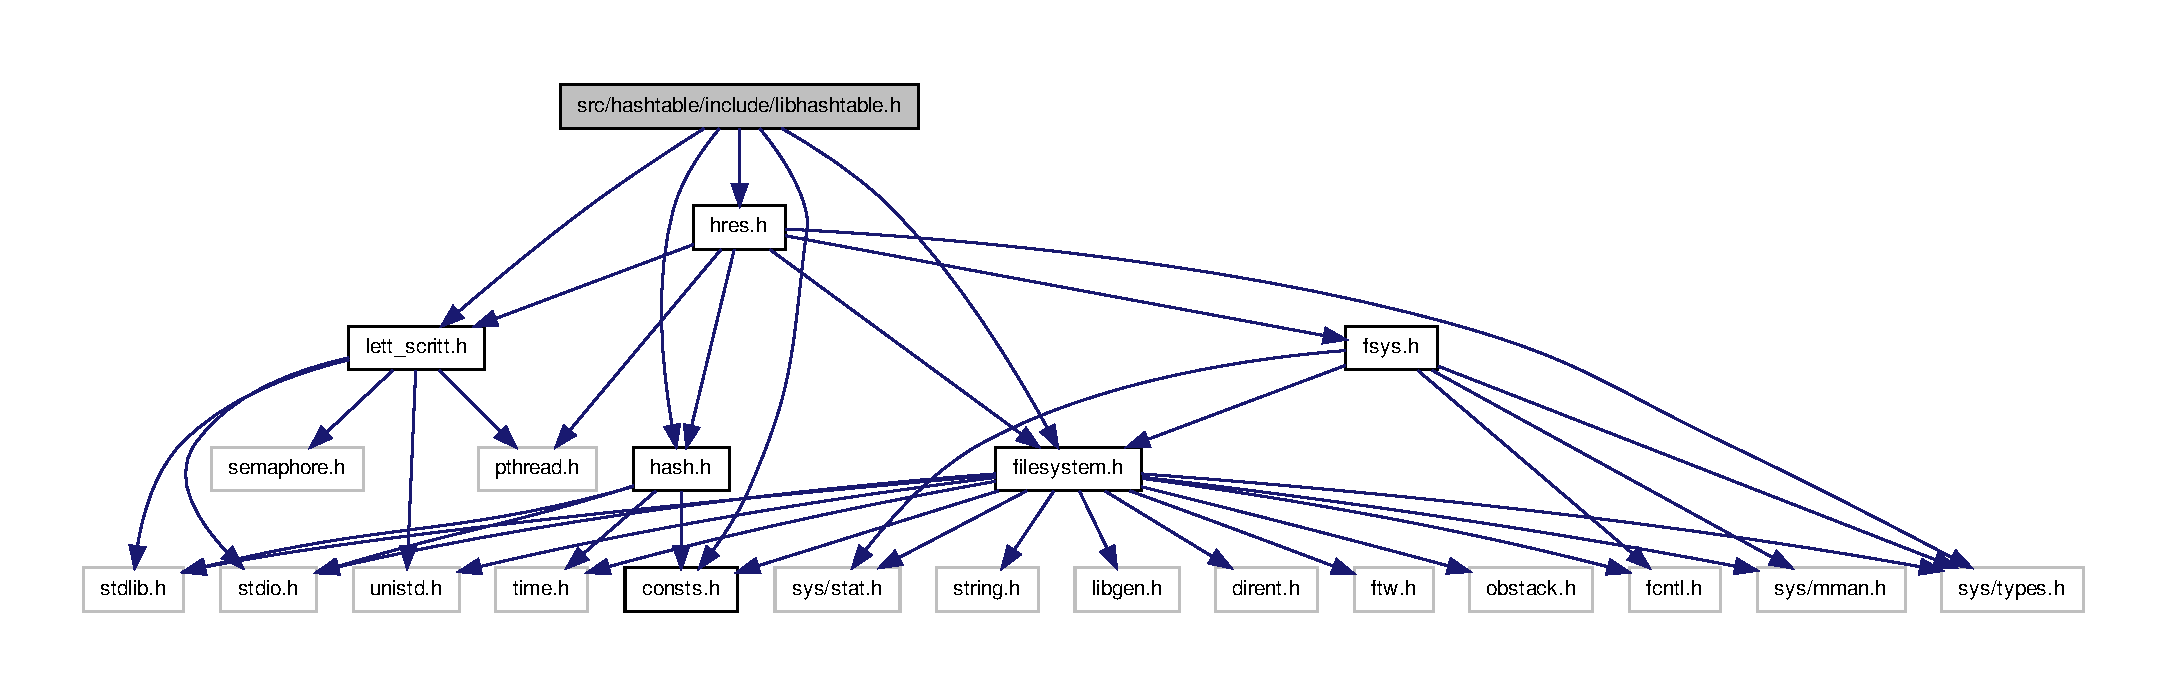
\includegraphics[width=400pt]{hashtable_2include_2libhashtable_8h__incl}
\end{center}
\end{figure}
Questo grafo mostra quali altri file includono direttamente o indirettamente questo file:
\nopagebreak
\begin{figure}[H]
\begin{center}
\leavevmode
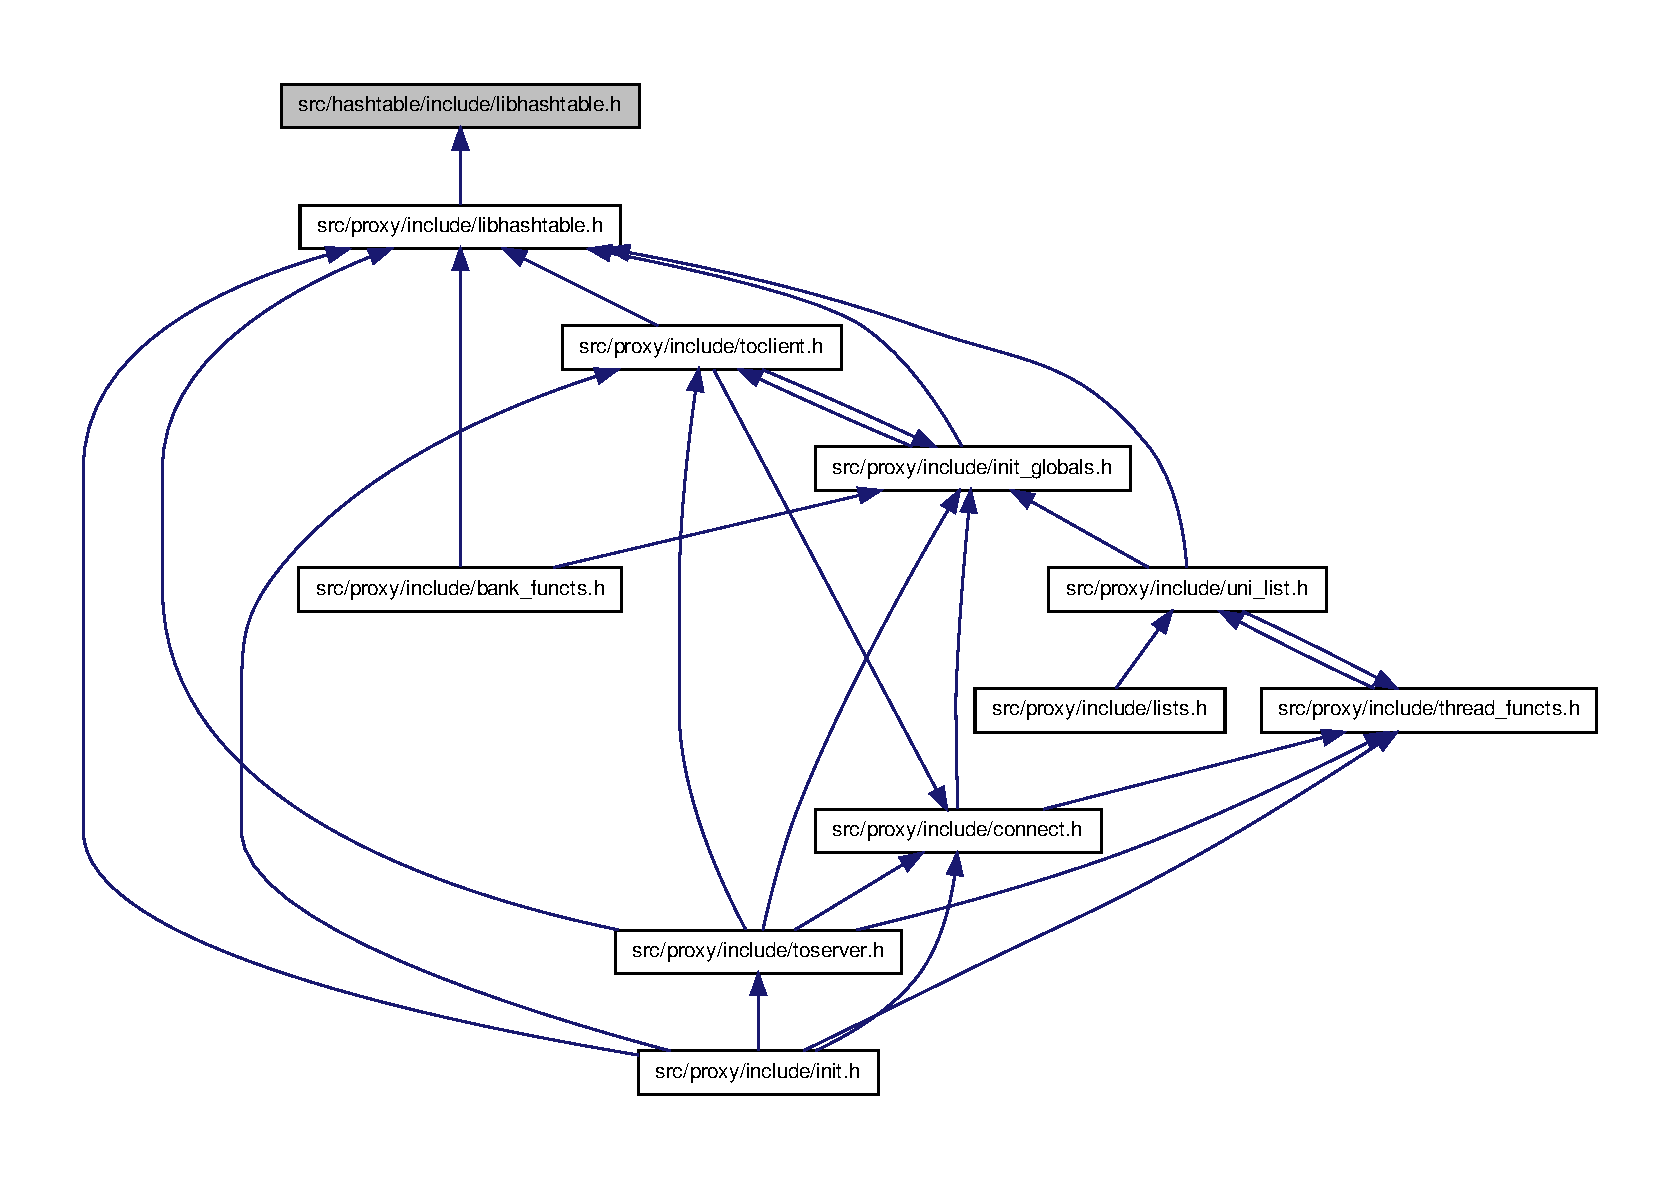
\includegraphics[width=400pt]{hashtable_2include_2libhashtable_8h__dep__incl}
\end{center}
\end{figure}
